\documentclass[11pt]{jarticle}
%
\usepackage[dvipdfmx]{graphicx}
\usepackage{amsmath}
\usepackage{amssymb}
\usepackage{bm}
\usepackage{latexsym}
\usepackage{float}
\usepackage{hyperref}
\usepackage{color}
\usepackage[justification=centering]{caption}
\usepackage{verbatim}
\usepackage{multicol}
\usepackage{listings}
%
\addtolength{\textwidth}{40mm}
\addtolength{\oddsidemargin}{-20mm}
\addtolength{\evensidemargin}{-20mm}
\addtolength{\textheight}{15mm}
\addtolength{\topmargin}{-10mm}
%
\renewcommand{\lstlistingname}{リスト}
%
\pagestyle{empty}
%
\title{研究進捗報告 \\ 付録}
\author{里谷 佳紀}
%\date{\today}
\date{平成29年10月3日}
%
\begin{document}
%
\maketitle
\thispagestyle{empty}
%
\appendix
\section{n=24,d=3で下界を達成するグラフ}
辺のリストをリスト\ref{list:edge}に,グラフを図\ref{fig:cerf-graph}
に示す.

\captionof{lstlisting}{辺リスト}
\label{list:edge}
\begin{multicols}{4}
  \verbatiminput{n24.naive_dfs_r2.elist}
\end{multicols}

\begin{figure}[H]
  \centering
  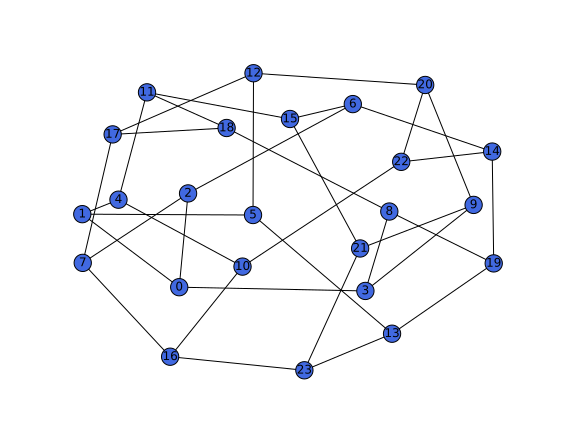
\includegraphics[width=.6\textwidth]{week3-graph-n24.pdf}
  \caption{n=24,d=3で下界を達成するグラフ}
  \label{fig:cerf-graph}
\end{figure}

\end{document}
